\documentclass[12pt, letterpaper, twoside]{article}
\usepackage[T2A]{fontenc}
\usepackage{amsfonts}
\usepackage{amsmath}
\usepackage{mathabx}
\usepackage{graphicx}
\usepackage{tikz}
\usepackage{pgfplots}

\pgfplotsset{compat = newest}

\title{Семинары по математическому анализу 4 модуль.}
\author{Андрей Тищенко}
\date{2023/2024}

\newcommand{\tg}{\operatorname{tg}}
\newcommand{\Bold}[1]{$\textbf{#1}$}
\newcommand{\Underl}[1]{$\underline{\text{#1}}$}
\newcommand{\BU}[1]{$\underline{\textbf{#1}}$}
\newcommand{\DS}{\displaystyle}
\newcommand{\tr}{\operatorname{tr}}
\newcommand{\Rg}{\operatorname{Rg}}
\newcommand{\Hom}{\operatorname{Hom}}
\newcommand{\oo}{\infty}
\newcommand{\arctg}{\operatorname{arctg}}
\newcommand{\Abs}[1]{\left| #1 \right|}
\newcommand{\grad}{\operatorname{grad}}

\begin{document}
    \maketitle
    \[\textbf{Семинар 4 апреля}\]
    \[\text{Сходимость функциональных последовательностей.}\]
    $\{f_n(x)\}_{n\in \mathbb{N}}\quad x\in E\\
    \forall x \in E \quad f_n(x)\xrightarrow[n\rightarrow \infty]{}f(x)$
    \begin{enumerate}
        \item[Номер 1.]
        \begin{enumerate}
            \item[a.] $f_n(x) = \dfrac{nx^2}{x + 3n + 2} = \dfrac{x^2}{\frac{x}{n} + 3 + \frac{2}{n}} \xrightarrow[n\rightarrow \infty]{} \dfrac{x^2}{3}$
            \item[c.] $f_n (x) = n(x^{\frac{1}{n}} - 1),\ E = [1;\ 3]\\
            x = 1\Rightarrow f_n(x) \xrightarrow[n\rightarrow \infty]{} 0\\
            \dfrac{e^y - 1}{y} \xrightarrow[y\rightarrow 0]{} 1\\
            f_n(x) = \dfrac{e^{\frac{1}{n} \ln x} - 1}{\frac{1}{n}\ln x}\ln x \xrightarrow[n\rightarrow \infty]{} \ln x$\\
            Итак, $f_n(x) \xrightarrow[n\rightarrow\infty]{} \ln x$ 
        \end{enumerate}
        \item[Определение:] $f_n(x) \underset{n\rightarrow \infty}{\rightrightarrows} f(x)$ на $E\Leftrightarrow \sup_{E} |f_n(x) - f(x)|\xrightarrow[n\rightarrow \infty]{} 0\\
        \forall \varepsilon > 0\ \exists N_{\varepsilon}\ \forall n > N_2\ \forall x \in E\ |f_n(x) - f(x)| < \varepsilon\Rightarrow\\ \Rightarrow \sup_E |f_n(x) - f(x)| \leq \varepsilon$
        \item[Номер 2.]
        \begin{enumerate}
            \item[a.] $f_n(x) = \dfrac{\operatorname{arctg}(nx)}{\sqrt{n + x}},\ E = [0,\ +\infty)\\
            f_n(x)\xrightarrow[n\rightarrow \infty]{} 0$ поточечно.\\
            $\left| \dfrac{\operatorname{arctg}(nx)}{\sqrt{n + x}} \right| < \left| \dfrac{\pi}{\sqrt{n}} \right| < \varepsilon$
            \item[b.] $f_n(x) = n\sin \frac{1}{nx},\ E = [1,\ +\infty)\\
            f_n(x) \sim n\cdot \dfrac{1}{nx} = \dfrac{1}{x}\Rightarrow f_n(x) \longrightarrow \dfrac{1}{x} = f(x)\\
            \left| n\left(\sin \dfrac{1}{nx} - \dfrac{1}{nx}\right) \right| = \dots\\
            \sin y = y - \dfrac{y^3}{6} + \dfrac{\sin c}{24}y^4\\
            \dots = \left| n\left( \dfrac{1}{nx} - \dfrac{1}{nx} - \dfrac{1}{(nx)^3 6} + \dfrac{\sin c}{24}\dfrac{1}{(nx)^4}\right) \right|\leq \dfrac{1}{6 n^2} + \dfrac{1}{24n^3} \xrightarrow[n\rightarrow \infty]{} 0$ (тут подставили $x = 1$, получив максимальное значение)
        \end{enumerate}
        \item[Номер 3.]
        \begin{enumerate}
            \item[a.] $f_n(x) = \dfrac{nx}{1 + n^2 x^2},\ E = [0;\ 1]\\
            f_n(x) \xrightarrow[n\rightarrow \infty]{} 0$\\
            Рассмотрим последовательность $x_n = \dfrac{1}{n}\Rightarrow\\
            \Rightarrow f_n(x_n) = \dfrac{n\frac{1}{n}}{1 + n^2\frac{1}{n^2}} = \frac{1}{2}$\\
            Как дополнительный пример рассмотрели:\\
            $x^n$ на $(0;\ 1)\xrightarrow[n\rightarrow \infty]{}0\\
            x_n = 1 - \frac{1}{n}\\
            f_n(x_n) = \left(1 - \frac{1}{n}\right)^n\xrightarrow[n\rightarrow\infty]{} \dfrac{1}{e}$ не сходится абсолютно.
            \item[b.] $f_n(x) = \ln \left( 3 + \dfrac{n^2 e^x}{n^4 + e^{2x}} \right),\ E = [0;\ +\infty)\\
            f(x) = \ln 3\\
            f_n(x) = \left| f_n(x) - f(x) \right| = \left| \ln \left(1 + \dfrac{n^2 e^x}{3(n^4 + e^{2x})}\right) \right|$\\
            Рассмотрим последовательность $x_n = \ln n^2$. Тогда\\
            $g_n(x_n) = \ln \left(1 + \dfrac{n^2 n^2}{3(n^4 + n^4)} \right) = \ln \dfrac{7}{6}$
        
        \end{enumerate}
        
    \end{enumerate}
    \[\textbf{Семинар 12 апреля} \]
    $f_n(x),\ x\in E$\\
    1. $f_n(x) \xrightarrow[n\rightarrow \infty]{} f(x)$ на $E$.\\
    2. Можно ли переставлять операторы $\DS \lim_{n\rightarrow \infty},\ \lim_{x\rightarrow x_0},\ \frac{d}{dx},\ \int\ dx$?\\
    То есть выполняется ли:
    \[\lim_{n\rightarrow \infty} \lim_{x\rightarrow x_0} f_n(x) \overset{?}{=} \lim_{x\rightarrow x_0}\lim_{n\rightarrow \oo} f_n(x)\]
    \[\lim_{n\rightarrow \oo} \frac{d}{dx} f_n(x) \overset{?}{=} \frac{d}{dx} \underset{f(x)}{\underbrace{\lim_{n\rightarrow \oo} f_n(x)}}\]
    $E = [0;\ 1],\ f_n(x) = x^n \longrightarrow g(x) \begin{cases}
        0,\ x\in [0;\ 1)\\
        1,\ x = 1
    \end{cases}$\\
    $\DS \lim_{n\rightarrow \oo}\lim_{x\rightarrow 1^-} f_n(x) = \lim_{n\rightarrow \oo} 1 = 1\\
    \lim_{x\rightarrow 1^-}\lim_{n\rightarrow \oo} f_n(x) = \lim_{x\rightarrow 1^-} g(x) = 0$\\
    $0\neq 1\Rightarrow$ это неверно.\\
    $f_n(x) \overset{E}{\rightrightarrows} f(x) \Leftrightarrow \DS \sup_{x\in E} |f_n(x) - f(x)|\xrightarrow[n\rightarrow \oo]{} 0$\\
    Ряды $\DS \sum_{n = 1}^{+\oo} u_n(x) = S(x)\\
    \sum_{n = 1}^{+\oo} n\cdot x^{n - 1} = \sum^{+\oo}_{n = 1} (x^n)' \overset{?}{=} \left(\sum_{n = 1}^{+\oo} x^n\right)'$\\
    $S_n(x) = \DS\sum_{k = 1}^{n} u_k(x) \overset{E}{\rightrightarrows} S(x)\Leftrightarrow\\
    \sup_{x\in E}\Leftrightarrow |S_n(x) - S(x)| \xrightarrow[n\rightarrow\oo]{}0\\
    \sup_{x\in E} |\sum_{k = n+1}^{+\oo} u_k(x)|\leq \sum_{k = n+ 1}^{+\oo} a_k\xrightarrow[n\rightarrow \oo]{}0$\\
    \begin{enumerate}
        \item[Признак Вейерштрассе:] Если $u_n(x)$ мажорируется последовательностью $a_n$: $\forall n\ |u_n(x)| \leq a_n$,\\
        тогда $\DS \sum_{n = 1}^{+\oo}a_n$ сходится, тогда $S_n(x) \overset{E}{\rightrightarrows} S(x)$ 
        \item[Задача 1.]
        \begin{enumerate}
            \item[a.] $u_n(x) = \frac{\arctg(n^2 x)\cdot \cos(\pi n x)}{n\sqrt{n}},\ E=\mathbb{R}\\
            |u_n(x)| \leq \frac{\pi}{2n^{\frac{3}{2}}}$, ряд $\DS \sum_{n = 1}^{+\oo}a_n$ сходится.\newpage
            \item[b.] $u_n(x) = e^{-n(x^2 + \sin x)},\ E = [1;\ +\oo)$\\
            $e^{-n(x^2 + \sin x)} < e^{-n}$, так как
        \end{enumerate}
            \[\begin{cases}
                x \geq \sqrt{2}:\ x^2 + \sin x \geq 2 + \sin x \geq 1\\
                1 \leq x < \sqrt{2}:\ \sin x > 0 \Rightarrow x^2 + \sin x > 1
            \end{cases}\]
    \end{enumerate}
    \[\text{Функциональные ряды}\]
    $\DS \sum_{n = 1}^{+\oo} C_n\cdot (\underset{t}{\underbrace{x - a}})^n \Rightarrow \sum_{k = 1}^{+\oo} C_n\cdot t^n$. Множество сходимости такого ряда имеет вид $(-R;\ R),\ R\in \overline{\mathbb{R}}$, $R$ называется \Underl{радиусом сходимости}.\\
    $R = \DS\lim_{n\rightarrow\oo} \Abs{\frac{C_n}{C_{n + 1}}}\\
    \frac{1}{R} = \lim_{n\rightarrow \oo} \sqrt[n]{|C_n|}$
    \begin{enumerate}
        \item[2.]
        \begin{enumerate}
            \item[a.] $\DS \sum_{n = 1}^{\oo} \frac{x^n}{n^2}\\
            R = \lim_{n\rightarrow \oo} \Abs{\frac{(n + 1)^2}{n^2}} = \lim_{n\rightarrow \oo}\Abs{\frac{n^2 + 2n + 1}{n^2}} = 1$
            \item[b.] $\DS \sum_{n = 1}^{\oo} \frac{x^n}{n!}\\
            R = \lim_{n\rightarrow \oo} \Abs{\frac{(n + 1)!}{n!}} = \lim_{n\rightarrow \oo} |n| = +\oo$
            \item[c.] $\DS \sum_{n = 1}^{\oo} 5^n x^{3n} = \sum_{n = 1}^{\oo} 5^n t^{n}\\
            \frac{1}{R_t} = \lim_{n\rightarrow \oo} \sqrt[n]{\Abs{5^n}}\Rightarrow \forall t: \Abs{t} < \frac{1}{5}\Rightarrow \Abs{x^3} < \frac{1}{5}\Rightarrow \Abs{x} < \frac{1}{\sqrt[3]{5}}\Rightarrow\\
            \Rightarrow R_x = \frac{1}{\sqrt[3]{5}}$
        \end{enumerate}
        \item[3.]
        \begin{enumerate}
            \item[a.] $\DS \sum_{n = 1}^{\oo} \frac{2n + 1}{3n^2 + 2}(x - 1)^n\\
            R = \lim_{m\rightarrow \oo} \frac{\frac{2n + 1}{3n^2 + 2}}{\frac{2n + 3}{3n^2 + 6n + 5}} = 1\Rightarrow (0;\ 2)$\\
            Рассмотрим граничные точки:\\
            $x = 2\Rightarrow \DS\sum_{n = 1}^{\oo} \frac{2n + 1}{3n^2 + 2} \sim \sum_{n = 1}^{\oo}\frac{2}{3n}$ расходится.\\
            $x = 0\Rightarrow \DS\sum_{n =1}^{\oo} (-1)^n \frac{2n + 1}{3n^2 + 2}$\\
            $\left( \frac{2n + 1}{3n^2 + 2} \right)' =  \frac{2(3n^2 + 2) - 6n(2n + 1)}{(3n^2 + 2)^2} = \frac{-6n^2 - 6n + 4}{(3n^2 + 2)^2}\Rightarrow$ с какого-то момента она монотонно убывает. Тогда по признаку Лейбница ряд сходится.
        \end{enumerate}
        \item[4.]
        \begin{enumerate}
            \item[a.] $\DS \sum_{n = 1}^{+\oo} nx^n = x\cdot \sum_{n = 1}^{+\oo} nx^{n - 1} = x\sum_{n = 1}^{+\oo} (x^n)' = x\left( \sum_{n = 1}^{+\oo} x^n \right) = x\cdot \left(\frac{x}{1 - x}\right)' =\\
            = x\frac{(1 - x) + x}{(1 - x)^2} = \frac{x}{(1 - x)^2}$\\
            Очевидно, что радиус сходимости такой функции равен $1$. Положим $x = \frac{1}{2}\Rightarrow \DS \sum_{n = 1}^{+\oo} \frac{n}{2^n} = ч \frac{\frac{1}{2}}{(1 - \frac{1}{2})^2} = 2$.
            \item[b.] $\DS \sum_{n = 0}^{\oo} \frac{(-1)^n}{x^{2n + 1}}{2n + 1} = \sum_{n = 0}^{\oo} \int_0^x (-1)^n t^{2n}\, dt = \int_0^x\sum_{n = 0}^{\oo} (-1)^n t^{2n}\, dt = \\
            = \int_0^x \sum_{n = 1}^{\oo} (-t^2)^n\, dt = \int_0^x \frac{1}{1 + t^2}dt = \arctg t |_0^x = \arctg x$
        \end{enumerate}
        \item[5.]
        \begin{enumerate}
            \item[a.] $\DS \sum_{n = 0}^{\oo} \frac{(-1)^n}{2n + 1}$
        \end{enumerate}
    \end{enumerate}
    \[\textbf{Семинар 26 апреля.}\]
    \begin{enumerate}
        \item[\textbf{Теория:}]
    \end{enumerate}
    \[f(\vec{x}): \mathbb{R}^{n}\rightarrow \mathbb{R},\ \lim_{\vec{x}\rightarrow \vec{x}_0} f(\vec{x}) = A\Leftrightarrow\]
    \[\Leftrightarrow\text{Коши: } \forall \varepsilon > 0\ \exists \delta > 0\ \forall \vec{x}\in \overset{\circ}{U}_{\delta}(\vec{x}_0)\ \ \Abs{f(\vec{x}) - A} < \varepsilon\]
    \[\Leftrightarrow\text{Гейне: } \forall \vec{x}_n \xrightarrow[n\rightarrow \oo]{} \vec{x}_0,\ \vec{x}_n \neq \vec{x}_0\Rightarrow f(\vec{x}_n)\xrightarrow[n\rightarrow \oo]{} A\]
    \begin{enumerate}
        \item[\textbf{Задача 1. a.}]
    \end{enumerate}
    \[\underset{y\rightarrow 1}{\lim_{x\rightarrow 2}}\, \frac{x^2 - 4y^2}{x^2 + 2x - 2xy - 4y} = \underset{y\rightarrow 1}{\lim_{x\rightarrow 2}}\, \frac{(x - 2y)(x + 2y)}{(x + 2)(x - 2y)} = \underset{y\rightarrow 1}{\lim_{x\rightarrow 2}}\, \frac{x + 2y}{x + 2} = 1\]
    \begin{enumerate}
        \item[\textbf{Задача 1. b.}]
    \end{enumerate}
    \[\underset{y\to 2}{\lim_{x\to 0}} \frac{\sin xy}{x} = \underset{y\to 2}{\lim_{x\to 0}} \underset{1}{\underbrace{\frac{\sin xy}{xy}}}y = 1\cdot 2 = 2\]
    \begin{enumerate}
        \item[\textbf{Задача 1. c.}]
    \end{enumerate}
    \[\underset{y\to 1}{\lim_{x\to 0}} (1 + x)^{\frac{1}{x + x^2y}} = \underset{y\to 1}{\lim_{x\to 0}} (1 + x)^{\frac{1}{x}\frac{1}{x + y}}= \underset{y\to 1}{\lim_{x\to 0}} \left( (1 + x)^{\frac{1}{x}} \right)^{\frac{1}{x + y}} = e^{\frac{1}{0 + 1}} = e\]
    \begin{enumerate}
        \item[\textbf{Задача 2.}]
    \end{enumerate}
    \[f(x,\ y) = \begin{cases}
        \dfrac{x^2 - y^2}{x^2 + y^2},\ x^2 + y^2 \neq 0\\
        a,\ \text{иначе}
    \end{cases}\]
    \begin{enumerate}
        \item[\textbf{a.}] Является непрерывной по $x$.
    \end{enumerate}
    $f(x,\ 0) = \begin{cases}
        \frac{x^2}{x^2},\ x^2 \neq 0\\
        a,\ x^2 = 0
    \end{cases},\ \DS \lim_{x\to 0} f(x,\ 0) = 1\Rightarrow a = 1$
    \begin{enumerate}
        \item[\textbf{b.}] Является непрерывной по $y$.
    \end{enumerate}
    $f(0,\ y) = \begin{cases}
        -\frac{y^2}{y^2},\ y^2 \neq 0\\
        a,\ y^2 = 0
    \end{cases},\ \DS \lim_{y\to 0} f(0,\ y) = -1\Rightarrow a = -1$
    \begin{enumerate}
        \item[\textbf{c.}] Является непрерывной по кривой $y = \alpha\sqrt{x},\ \alpha \neq 0$ 
    \end{enumerate}
    $f(x,\ \alpha\sqrt{x}) = \begin{cases}
        \frac{x^2 - \alpha x}{x^2 + \alpha^2 x},\ x^2 + \alpha x \neq 0\\
        a,\ x^2 + \alpha^2 x = 0
    \end{cases},\DS \lim_{x\to 0} \frac{x^2 - \alpha^2 x}{x^2 + \alpha^2 x} = \frac{x - \alpha^2}{x + \alpha^2} \xrightarrow[x\to 0]{} -1 = a$
    \begin{enumerate}
        \item[\textbf{d.}] Является $https://de.pornhub.com/$ непрерывной.
    \end{enumerate}
    Ни при каких, так как уже при приближении по $x$ и по $y$ значения параметра $a$ для достижения непрерывности должны различаться.
    \begin{enumerate}
        \item[\textbf{Задача 3.}] Вычислить пределы:
    \end{enumerate}
    \begin{enumerate}
        \item[\textbf{a.}]
    \end{enumerate}
    \[f(x,\ y) = \frac{x^2 y}{x^2 + y^2}\]\newpage
    \[\lim_{x\to 0}\lim_{y \to 0} f(x,\ y) = \lim_{x\to 0} \frac{0}{x^2} = \lim_{x\to 0} 0 = 0\]
    \[\lim_{y\to 0}\lim_{x\to 0} f(x,\ y) = 0,\ \text{аналогично}\]
    \[\underset{y\to 0}{\lim_{x\to 0}}\, \frac{x^2 y}{x^2 + y^2}\]
    Знаем $\forall \varepsilon > 0\ \exists \delta > 0\ \underset{\sqrt{x^2 + y^2} < \delta\Rightarrow |x|<\delta}{\forall (x,\ y)\in \overset{\circ}{U}_{\delta}(0,\ 0)}\ \underset{\Abs{\frac{x^2 y}{x^2 + y^2}} < \varepsilon}{\Abs{f(x,\ y) - 0} < \varepsilon}$\\
    Также знаем $\frac{x^2 + y^2}{2} \geq xy\Rightarrow \Abs{\frac{x^2 y}{x^2 + y^2}} \leq \Abs{\frac{x}{2}} < \Abs{\frac{\delta}{2}}\leq\varepsilon$. Верно при $\delta = 2\varepsilon$
    \begin{enumerate}
        \item[\textbf{b.}]
    \end{enumerate}
    \[f(x,\ y) = x + y\sin \frac{1}{y}\]
    \[\lim_{x\to 0}\lim_{y\to 0} x + y\sin \frac{1}{y} = \lim_{x\to 0} x = 0\]
    \[\lim_{y\to 0}\lim_{x\to 0} x + y\sin\frac{1}{y} = \lim_{y\to 0} y\sin \frac{1}{y} = 0\]
    Скорее всего ошибка в задании, так как слагаемые сходятся внезависимости друг от друга, дальше не решали.
    \begin{enumerate}
        \item[\textbf{c.}]
    \end{enumerate}
    \[f(x,\ y) = \log_{1 + x}(1 + x + y)\]
    \[\lim_{x\to 0}\lim_{y\to 0} \log_{1 + x}(1 + x + y) = \lim_{x\to 0} \log_{1 + x}(1 + x) = 1\]
    \[\lim_{y\to 0}\lim_{x\to 0} \log_{1 + x}(1 + x + y) = \lim_{y\to 0}\lim_{x \to 0} \frac{\ln(1 + x + y)}{\ln(1 + x)} = \oo\]
    Дробь стремится к бесконечности, значит переходить к пределу по $y$ переходить нельзя. Пределы не совпадают, значит к многомерному пределу переходить нельзя\newpage
    \begin{enumerate}
        \item[\textbf{Вставка:}]
    \end{enumerate}
    $\underset{\Updownarrow}{\text{Открытость множества $A$}}$ $\longleftrightarrow$ метрика $\longrightarrow$ шары или окрестность.\\
    $\forall x\in A\ \exists \delta\ U_{\delta}(x)\subset A$\\
    Замкнут $\Leftrightarrow$ дополнение к открытости.
    \begin{enumerate}
        \item[\textbf{1.}] Свойства непрерывных на компакте
    \end{enumerate}
    Компакт $\overset{\mathbb{R}^n}{\Longleftrightarrow}$ ограниченность, замкнутость.
    \begin{enumerate}
        \item[\textbf{2.}] $f$ непрерывна на $E\Leftrightarrow\\
        \Leftrightarrow \underset{\{x\, |\, f(x)\in A\}}{f^{-1}(A)}$ - открытый для любого открытого $A$
    \end{enumerate}
    \begin{enumerate}
        \item[\textbf{Задача 4.}]
    \end{enumerate}
    $f$ - непрерывна. $A = \{x\, |\, f(x) > y_0\}$\\
    Пусть $x_1\in A\ f(x_1) > y_0$. Возьмём $\varepsilon_0 = \dfrac{f(x_1) - y_0}{2}$, тогда из определения непрерывности:\\
    $\exists \delta > 0\ \forall x\in \overset{\circ}{U}_{\delta}(x_1)\ \Abs{f(x) - f(x_1)} < \varepsilon_0\Rightarrow f(x) > y_0$, ч.т.д.\\
    Вторую часть задачи решили устно (несложное упражнение).
    \begin{enumerate}
        \item[\textbf{Задача 5.}]
    \end{enumerate}
    \begin{enumerate}
        \item[\textbf{Определение:}]
    \end{enumerate}
    Точка $x$ называется граничной точкой множества $A$, если:
    \[\forall \delta>0\ \exists x_0 \in U_{\delta}(x)\ x_0\in A \wedge \exists x_1 \in U_{\delta}(x)\ x_1 \in \overline{A}\]
    \[\textbf{Семинар 10 мая}\]
    Рассматриваем такие штуки: $f(\vec{x}): \mathbb{R}^n \to \mathbb{R}$
    \begin{enumerate}
        \item[0.] Определение, множество значений, линии уровня.
        \item[1.] $\DS \lim_{\vec{x}\to \vec{x}_0} f(\vec{x}) = A$.  
    \end{enumerate}
    Гейне:
    \[\forall \vec{x}_n\xrightarrow[n\to \oo]{} \vec{x}_0\quad \vec{x}_n \neq \vec{x}:\ f(\vec{x}_n)\xrightarrow[n\to\oo]{} A\]
    $\DS \lim_{\vec{x}\to \vec{x}_0} f(\vec{x}) = f(\vec{x}_0)$
    \[\forall i\ x_n^i\xrightarrow[n\to\oo]{} x_0^i \Leftrightarrow \rho(\vec{x}_n;\ \vec{x}_0)\xrightarrow[n\to\oo]{} 0,\quad \sum_{i = 1}^{n} \Abs{x^i_n - x^i_0}^2\to 0\]
    \begin{enumerate}
        \item[2.] Дифференцируемость
    \end{enumerate}
    В одномерном случае:
    \[f'(x_0) = \lim_{x\to x_0} \frac{f(x) - f(x_0)}{x - x_0} \Leftrightarrow f(x) = f(x_0) + A(x - x_0) + \overline{o}(x - x_0)\]
    В многомерном:\\
    Определение: $f(x)$ называется дифференцируемой в точке $\vec{x}_0$:
    \[f(\vec{x}) = f(\vec{x}_0) + \sum_{i = 1}^{n} A_i(x^i - x_0^i) + \overline{o}\big(\rho(\vec{x};\ \vec{x}_0)\big)\]
    Определение: $\DS\frac{\vartheta f}{\vartheta x_i} = \lim_{x^i\to x^i_0} \frac{f(x_0^i),\dots,\ x^i,\dots,\ x_0^i - f(\vec{x}_0)}{x^i - x^i_0}$\\
    Пример:\\
    $f(x,\ y) = \dfrac{xy}{x^2 + y^2}\\
    f(x,\ 0) = \frac{0}{x^2}\\
    \dfrac{\vartheta f(x,\ 0)}{\vartheta x} = 0\quad \dfrac{\vartheta f(0,\ y)}{\vartheta y} = 0$
    \[\text{Достаточное условие дифференцируемости}\]
    \begin{enumerate}
        \item[1.] $\dfrac{\vartheta f}{\vartheta x_i}\ \exists$ окрестность точки $\vec{x}_0$
        \item[2.] Частные производные в точке $\vec{x}_0$ непрерывны\\
        $\Rightarrow$ функция дифференцируема в точке $\vec{x}_0$
    \end{enumerate}
    \begin{enumerate}
        \item[\textbf{Задача 1.}]
    \end{enumerate}
    $f(x,\ y) = x + y^2 + \ln(x + y^2)\\
    \frac{\vartheta f(x,\ y)}{\vartheta x} = 1 + \frac{1}{x + y^2}\quad \frac{\vartheta f(x,\ y)}{\vartheta y} = 2y + \frac{2y}{x + y^2}$\\
    В окрестности точки $(0,\ 1)$ существуют частные производные (так как точка лежит в области определения).\\
    $(x_n,\ y_n)\to (0,\ 1)$, непрерывность есть, так как частные производные непрерывны на области определения, значит функция дифференцируема.\\
    $df(x,\ y)\big|_{\overset{x = 0}{y=0}} = 2dx + 4dy$
    \begin{enumerate}
        \item[\textbf{Задача 2. a.}]
    \end{enumerate}
    $f(x,\ y) = \sqrt[3]{xy}\\
    \frac{\vartheta f}{\vartheta x} = \sqrt[3]{y}\frac{1}{3\sqrt[3]{x}},\quad \frac{\vartheta f}{\vartheta y} = \sqrt[3]{x}\frac{1}{3\sqrt[3]{y}}\\
    \frac{\vartheta f}{\vartheta x}\frac{\vartheta f}{\vartheta y}\big|_{\overset{x=0}{y=0}} = 0$.\\
    Очевидно:\\
    $f(x,\ 0) \equiv 0\ \forall x\\
    f(0,\ y) \equiv 0\ \forall y\\
    \sqrt[3]{xy} = 0 + Ax + By + \overline{o}(\sqrt{x^2 + y^2})$\\
    При этом $A,\ B$ являются частными производными, то есть
    $\sqrt[3]{xy} = \overline{o}(\sqrt{x^2 + y^2})\\
    \dfrac{\sqrt[3]{xy}}{\sqrt{x^2 + y^2}}\xrightarrow[(x,\ y)\to(0,\ 0)]{}0$\\
    Положим $x = y\Rightarrow \dfrac{\sqrt[3]{x^2}}{\sqrt{2x^2}} = \frac{1}{\sqrt{2}}\frac{1}{\sqrt[3]{x}}\xrightarrow[x\to 0]{} \infty$, то есть дифференцируемости нет.
    \begin{enumerate}
        \item[\textbf{Задача 2. b.}]
    \end{enumerate}
    $f(x,\ y) = \cos \sqrt[3]{xy}\\
    \frac{\vartheta f(x,\ y)}{\vartheta x} = -\sin \sqrt[3]{xy}\cdot \frac{\sqrt[3]{y}}{3\sqrt[3]{x^2}}\\
    \frac{\vartheta f(x,\ y)}{\vartheta y} = -\sin \sqrt[3]{xy}\cdot \frac{\sqrt[3]{x}}{3\sqrt[3]{y^2}}$\\
    Частные производные есть, в точках $(x,\ 0)$ и $(0,\ y)$ они равны 0, так как синус обратится в тождественную 1.\\
    $\cos \sqrt[3]{xy} = 1 + Ax + By + \overline{o}(\rho(x,\ y))\\
    \cos\sqrt[3]{xy} - 1 = \overline{o}(\sqrt{x^2 + y^2})\\
    \dfrac{\cos \sqrt[3]{xy} - 1}{\sqrt{x^2 + y^2}} = \dfrac{-\frac{\sqrt[3]{x^2y^2}}{2} + \overline{o}(1)(\sqrt[3]{x^2y^2})}{\sqrt{x^2 + y^2}}\leq \dots$\\
    Из неравенства Коши $\sqrt{x^2 + y^2} \geq \sqrt{2xy}\\
    \dots \leq \dfrac{-\frac{(xy)^{\frac{2}{3}}}{2} + \overline{o}(1)(\sqrt[3]{xy})^2}{\sqrt{2xy}} \xrightarrow[(x,\ y)]{} 0$
    \begin{enumerate}
        \item[\textbf{Задача 3.}]
    \end{enumerate}
    $f(u,\ v),\ f_u'\ f'_v\\
    g(x,\ y) = f(x\cos y,\ x\sin y)\\
    \dfrac{\vartheta g}{\vartheta x} = \dfrac{df}{du}\dfrac{du}{dx} + \dfrac{df}{dv}\dfrac{dv}{dx} = f'_u(x\cos y)'_x + f'_v (x\sin y)'_x = f'_u \cos y + f'_v \sin y$\\
    \[\text{Производная по направлению}\]
    $\vec{e}(e_1,\dots,\ e_n),\ \Abs{\vec{e}} = 1\\
    f(\vec{x}_0 + t\vec{e}) = g(t)$
    \[\textbf{Семинар 17 мая.}\]
    \subsubsection*{Задача 5.}
    $\arctg \frac{xy}{z^2},\ M(0;\ 1;\ 2)\\
    \overrightarrow{grad\ f} = \overrightarrow{\varbigtriangledown\ f} = (\frac{1}{4};\ 0;\ 0)\\
    1.\ \frac{\vartheta f}{\vartheta x} = \frac{1}{\left(\frac{xy}{z^2}\right)^2 + 1}\cdot \frac{y}{z^2}\big|_{M} = \frac{1}{4}\\
    2.\ \frac{\vartheta f}{\vartheta y} = \frac{1}{\left(\frac{xy}{z^2}\right)^2 + 1}\cdot \frac{x}{z^2}\big|_{M} = 0\\
    3.\ \frac{\vartheta f}{\vartheta z} = \frac{1}{\left(\frac{xy}{z^2}\right)^2 + 1}\cdot \frac{-2}{z^3}xy\big|_{M} = 0$
    \subsubsection*{Задача 4.}
    $f(x,\ y,\ z) = x^3 + 2xy^2 + 3yz^2\\
    \vec{l} = (2,\ 2,\ 1),\ M = (3,\ 3,\ 1)\\
    \frac{\vartheta f}{\vartheta x} = 3x^2 + 2y^2\\
    \frac{\vartheta f}{\vartheta y} = 4xy + 3z^2\\
    \frac{\vartheta f}{\vartheta z} = 6yz\\
    \overrightarrow{\varbigtriangledown\ f} = (45,\ 39,\ 18)\\
    \vec{l}_n = \frac{(2,\ 2,\ 1)}{\sqrt{9}} = \left(\frac{2}{3},\ \frac{2}{3},\ \frac{1}{3}\right)\\
    \frac{\vartheta f}{\vartheta l_n} = 30 + 26 + 6 = 62$ (скалярное произведение векторов $\vec{l}_n,\ \overrightarrow{\varbigtriangledown\ f}$)\\
    \subsubsection*{Задача 6.}
    $f(x,\ y) = x^2 + y^2$. Возьмём произвольную точку $(x_0,\ y_0)$. Тогда возьмём вектор единичного размера:
    \[\vec{n} = \left\{ \frac{x_0}{\sqrt{c}},\ \frac{y_0}{\sqrt{c}} \right\}\]
    Посчитаем частные производные:\\
    $\frac{\vartheta f}{\vartheta x} = 2x,\ \frac{\vartheta f}{\vartheta y} = 2y\Rightarrow \overrightarrow{\varbigtriangledown f} = (2x_0;\ 2y_0)$
    \[\textbf{Неявно заданные функции}\]
    $F(y,\ \vec{x}) = 0$
    \subsubsection*{Задача 2. а.}
    Рисуночки, ура.
    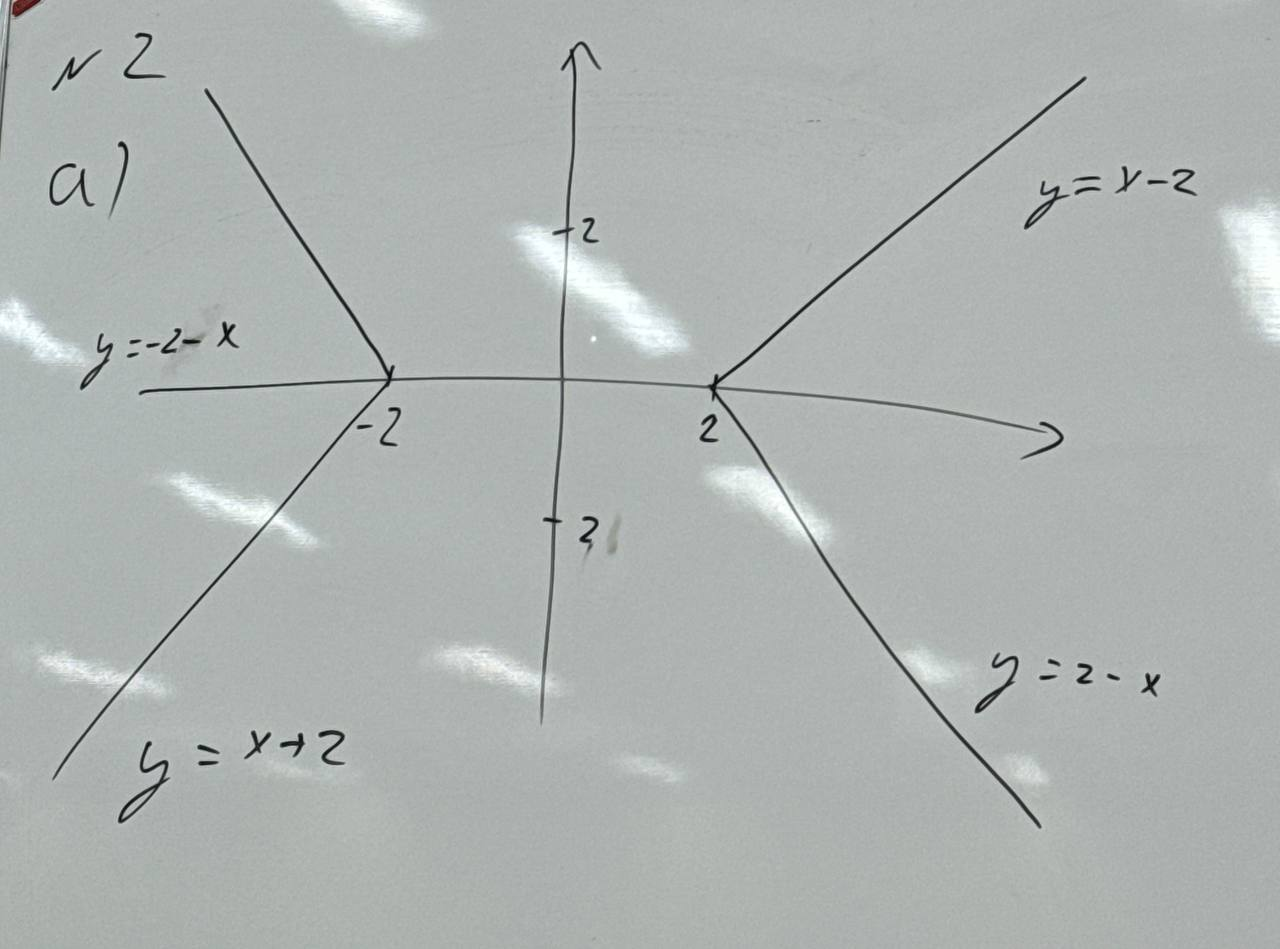
\includegraphics[width=0.5\linewidth]{../pictures/Graph a.jpg}
    \subsubsection*{Задача 2. b.}
    \subsubsection*{Задача 2. c.}

\[\textbf{Семинар 24 мая}\]
    \subsubsection*{Задача 4.}
    $x + y(x) = xy^2(x) - x^2y(x),\quad |y| < |x|$\\
    Продифференцируем по $x$: $1 + y_x' = y^2 + 2xy\cdot y_x' - x^2y'_x - 2xy\Rightarrow\\
    \Rightarrow y'_x = \dfrac{y^2-2xy-1}{1 - 2xy + x^2} = 0,\ |y| < |x|\\
    \begin{cases}
        \dfrac{y^2-2xy-1}{1 - 2xy + x^2} = 0\\
        x + y = xy^2 - x^2y
    \end{cases}\\
    x = \dfrac{y^2 - 1}{2y}\\
    x + y = x y^2 - x^2 y\\
    \frac{y^2 - 1}{2y} + y = \frac{y^2 - 1}{2y}y^2 - \left(\frac{y^2 - 1}{2y}\right)y$\\
    Решение системы было подсказано:\\
    $y = \pm\sqrt{3 \pm 2\sqrt{2}}$\\
    Вспоминаем факты из прошлого:\\
    $\begin{cases}
        y_x' = 0\\
        y''_{xx} > 0
    \end{cases}$ - точка минимума\\
    $\begin{cases}
        y_x' = 0\\
        y''_{xx} < 0
    \end{cases}$ - точка максимума\\
    Дифференцируем второй раз (при этом в наших точках первая производная зануляется):\\
    $y_{xx}'' - 2y_{xx}''xy + x^2y_{xx}'' = -2y - \underset{=0}{2xy'_x}\\
    y_{xx}'' = \dfrac{-2y}{1 - 2xy + x^2} = \dfrac{2y}{2xy - 1 - x^2}$
    \subsubsection*{Задача 5.}
    Хотим $u = f(x,\ y)$. \[u^3 - 2u^2x + uxy - 2 = 0\] Выясним, выполняется ли теорема о неявной функции.
    \[\frac{\vartheta F}{\vartheta u} = 3u^2 - 4ux + xy\big|_{\underset{y = 1}{x = 1}} = 3u^2 - 4u + 1\]
    Найдём $u$ с помощью изначального уравнения, подставив $\begin{cases}
        x = 1\\
        y = 1
    \end{cases}$:
    \[u^3 - 2u^2 + u - 2 = (u - 2)(u^2 + 1)\Rightarrow u = 2\]
    Тогда $\dfrac{\vartheta F}{\vartheta u} = 12 - 8 + 1 = 5\neq 0$\\
    $F(u,\ x,\ y) = 0\longrightarrow u = u(x,\ y)$\\
    Тогда изначальное равенство выглядит так:
    \[(*) = u^3(x,\ y) - 2u^2(x,\ y)x + u(x,\ y)xy - 2 = 0\]
    \[\frac{\vartheta (*)}{\vartheta x} = 3u^2u'_x - 4uu_x'x - 2u^2 + u_x'xy + uy = 0\]
    Подставим найденное значение $u$ и заданные значения $x,\ y$:
    \[12u'_x - 8u'_x - 8 + u'_x + 2 = 0\Rightarrow u_x' = \frac{6}{5}\]
    \subsubsection*{Задача 6.}
    Найти в точке $(x,\ y,\ u,\ v) = (1,\ 0,\ 1,\ -2)$ частные производные\\
    $u = f_1(x,\ y),\ v = f_2(x,\ y)$, заданной системой:
    \[\begin{cases}
        xu + yv - u^3 = 0\\
        x + y + u + v = 0
    \end{cases}\]
    Хотим, чтобы определитель матрицы Якоби не занулялся, то есть
    \[\begin{vmatrix}
        \dfrac{\vartheta F}{\vartheta u} & \dfrac{\vartheta F}{\vartheta v}\\
        \dfrac{\vartheta G}{\vartheta u} & \dfrac{\vartheta G}{\vartheta v}
    \end{vmatrix} \neq 0\Rightarrow \begin{vmatrix}
        x - 3u^2 & y\\
        1 & 1
    \end{vmatrix} = \begin{vmatrix}
        -2 & 0\\
        1 & 1
    \end{vmatrix} = -2\]
    Продолжаем решение:\\
    $\begin{cases}
        xu(x,\ y) + yv(x,\ y) - u^3(x,\ y) = 0\\
        x + y + u(x,\ y) + v (x,\ y) = 0
    \end{cases}$\\
    Дифференцируем по $y$:
    \[\begin{cases}
        xu_y' + v_y + v_y' y - 3u^2u_y' = 0\\
        u_y' + v_y' + 1 = 0
    \end{cases}\]
    Подставим значения $(1,\ 0,\ 1,\ -2)$
    \[\begin{cases}
        u'_y - 2 - 3u_y' = 0\\
        u'_y + v'_y + 1 = 0
    \end{cases}\Rightarrow \begin{cases}
        u'_y = -1\\
        v_y' = 0
    \end{cases}\]
    
\[\text{Нахождение экстремумов.}\]
    $\vec{x}_0$ называется точкой минимума, если $f(\vec{x}_0)$ самое маленькое в $U_{\delta}(\vec{x}_0)$
    \subsubsection*{Задача 1.}
    $u(x,\ y) = x^3 + 3xy^2 - 3yx - 36y + 26,\ \frac{\vartheta u}{\vartheta x} = 3x^2 + 3y^2 - 39,\ \frac{\vartheta u}{\vartheta y} = 6xy - 36 = 0\Rightarrow$
    \[\begin{cases}
        x^2 + y^2  =13\\
        xy = 6
    \end{cases}\Rightarrow \begin{cases}
        x = 2\\
        y = 3
    \end{cases}\vee \begin{cases}
        x = 3\\
        y = 2
    \end{cases}\vee \begin{cases}
        x = -3\\
        y = -2
    \end{cases}\vee \begin{cases}
        x = -2\\
        y = -3
    \end{cases}\]
    Составим матрицу Геса: $\begin{pmatrix}
        u''_{xx} & u_{xy}''\\
        u_{xy}'' & u_{yy}''
    \end{pmatrix} = \begin{pmatrix}
        6x & 6y\\
        6y & 6x
    \end{pmatrix}$\\
    Если матрица Геса положительно определена $\Rightarrow \vec{x}_0$ - точка минимума.\\
    Если она отрицательно определена $\Rightarrow \vec{x}_0$ - точка максимума.\\
    Если она знакопеременна $\Rightarrow \vec{x}_0$ - не экстремум.\\
    Итак, можно сделать вывод:\\
    $\begin{cases}
        x = 2\\
        y = 3
    \end{cases}$ - не экстремум\\
    $\begin{cases}
        x = 3\\
        y = 2
    \end{cases}$ - максимум\\
    $\begin{cases}
        x = -2\\
        y = -3
    \end{cases}$ - не экстремум\\
    $\begin{cases}
        x = -3\\
        y = -2
    \end{cases}$ - минимум\\

\[\textbf{Семинар 31 мая}\]
\subsubsection*{Задача 1.}
Найти условные экстремумы функции $u = xyz$ относительно уравнений связи
\[x + y + z = 6\hspace{1cm} x + 2y  + 3z = 6\]
Получаем систему:\\
$\begin{cases}
    u = xyz\\
    6 - y - 2z = 6\\
    y = 6 - 2y - 3z
\end{cases}\Leftrightarrow \begin{cases}
    u = z(-2z)(6 + z) = -2z^3 - 12z^2\\
    y = -2z\\
    x = 6 + z
\end{cases}\Rightarrow u' = -6z^2 - 24z = -6z(z + 4)$\\
То есть минимум при $z = -4$, максимум при $z = 0$
Ответ: точка минимума $(2,\ 8,\ -4)$, точка максимума $(6,\ 0,\ 0)$
\subsubsection*{Задача 2.}
Найти условные экстремумы функции $f(x,\ y) = 6 - 5x - 4y$ относительно уравнения связи:
\[x^2 - y^2 - 9 = 0\]
Если явно не выражается, то нужно составлять функцию Лагранжа:
\[L(\vec{x},\ \vec{\lambda}) = f_0(\vec{x}) + \sum_{i = 1}^{m} \lambda_i f_i(x)\]
$f_i$ - уравнение связи. $\lambda_i$ - коэффициенты для зануления набора $f_i$ (уравнения связи линейно зависимы)\par
Если $\vec{x}_0$ - точка условного локального экстремума, то $\exists \vec{\lambda}_0$\\
$\begin{cases}
    \left. \dfrac{\vartheta L}{\vartheta x_i} \right|_{\underset{\vec{\lambda}_0}{\vec{x}}} = 0\\
    f_i (\vec{x}_0) = 0
\end{cases}$  \\
Составим уравнение Лагранжа:\\
$6 - 5x - 4y = f(x,\ y)\\ x^2 - y^2 - 9 = 0\\
L(\vec{x},\ \vec{\lambda}) = 6 - 5x - 4y + \lambda(x^2 - y^2 - 9)\\
\dfrac{\vartheta L}{\vartheta x} = -5 + 3\lambda x = 0\\
\dfrac{\vartheta L}{\vartheta y} = -4 - 2\lambda y = 0\\
\begin{cases}
    -5 + 3\lambda x = 0\\
    -4 - 2\lambda y = 0\\
    x^2 - y^2 = 9
\end{cases}\Rightarrow \begin{cases}
    x = \dfrac{5}{2\lambda}\\
    y = -\dfrac{4}{2\lambda}\\
    \dfrac{25}{4\lambda^2} - \dfrac{16}{4\lambda^2} = 9\hspace{1cm} (1)
\end{cases}\\
(1): \dfrac{1 - 4\lambda^2}{4\lambda^2} = 0\Rightarrow \lambda = \pm \dfrac{1}{2}\Rightarrow \left[ \begin{gathered}
    \begin{cases}
        x = 5\\
        y = -4\\
        \lambda = \dfrac{1}{2}
    \end{cases}\\
    \begin{cases}
        x = -5\\
        y = 4\\
        \lambda = -\dfrac{1}{2}
    \end{cases}
\end{gathered} \right.$\\
Посчитаем Гессониан для каждой из $\lambda$:
\[\Gamma = \begin{pmatrix}
    2\lambda & 0\\
    0 & -2\lambda
\end{pmatrix}\]
Тогда для $\lambda = \dfrac{1}{2}$: $\begin{pmatrix}
    1 & 0\\
    0 & -1
\end{pmatrix}\Rightarrow$ не является экстремумом, так как знакочередующаяся (начиная с плюса).\\
Для $\lambda = -\dfrac{1}{2}$: $\begin{pmatrix}
    -1 & 0\\
    0 & 1
\end{pmatrix}\Rightarrow$ не является экстремумов, так как оба минора отрицательные.
\subsubsection*{Задача 3. a.}
Найти наибольшее и наименьшее значение функции на множестве заданном ограничением:
\[f(x,\ y) = (y^2 - x^2)\cdot e^{1 - x^2 + y^2}\hspace{1cm} x^2 + y^2 \leq 4\]
$\dfrac{\vartheta f}{\vartheta x} = (-2x)e^{1 - x^2 + y^2} + (y^2 - x^2)(-2x)e^{1 - x^2 + y^2} = 0\\
\dfrac{\vartheta f}{\vartheta y} = (2y)e^{1 - x^2 + y^2} + (y^2 - x^2)2ye^{1 - x^2 + y^2} = 0\\
\begin{cases}
    e^{1 - x^2 + y^2}(2y + 2y^3 - 2yx^2) = 0 \\
    e^{1 - x^2 + y^2}(-2x + 2x^3 - 2xy^2) = 0
\end{cases}\Leftrightarrow\begin{cases}
    y(y^2 - x^2 + 1) = 0\\
    x(x^2 - y^2 - 1) = 0
\end{cases}$\\
При $y = 0$: $\left[\begin{gathered}
    x = 1\\
    x = -1\\
    x = 0
\end{gathered}\right.$.\\
При $x = 0$: $y = 0$\\
При $x,\ y \neq 0$:
$x^2 - y^2 - 1 = 0\Rightarrow x^2 = y^2 + 1$\\
Рассмотрим значения функции от $x^2 - y^2$ при таких значениях\\
(не забываем про $x^2 + y^2 \leq 4$).
\[f(0) = e\cdot 0 = 0\]
\[f(1) = -1\]
Рассмотрим граничные точки:\\
$f_0(x,\ y) = (y^2 - x^2)e^{1 - x^2 + y^2} = 0\\
f_1(x,\ y) = x^2 + y^2 - 4 = 0\Rightarrow y^2 = 4 - x^2\\
f_0(x) = (4 - 2x^2)e^{5 - 2x^2}\Rightarrow f_0'(x) = -4xe^{5 - 2x^2} - 4x(4 - 2x^2)e^{5 - 2x^2} =\\
= e^{5 - 2x^2}(-4x)(1 + 4x - 2x^2) = 0\Rightarrow \left[ \begin{gathered}
    x = 0\\
    x = \pm \sqrt{\frac{5}{2}}
\end{gathered} \right.\Rightarrow\\
\Rightarrow f_0(0) = 4e^5,\ f\left(\pm \sqrt{\dfrac{5}{2}}\right) = -1e^0 = -1$\\
Стоит поверить desmos'у наслово, что точки $(0,\ \pm 1)$ являются локальными максимумами, а точки $\left(\sqrt{\frac{5}{2}},\ 0\right)$ - локальные минимумы.

\subsubsection*{Задача 3. b.}
\[f(x,\ y) = 3 + 2xy\hspace{1 cm} f_1(x,\ y) = x^2 + y^2 \leq 1\]
$\dfrac{\vartheta f}{\vartheta x} = 2y\\
\dfrac{\vartheta f}{\vartheta t} = 2x$\\
Зануляется в точке $0,\ 0$. $f(0,\ 0) = 3\\
:(\vec{x},\ \vec{\lambda}) = 3 + 2xy + \lambda(x^2 + y^2 - 1)\\
\dfrac{\vartheta L}{\vartheta x} = 2y + 2\lambda x = 0\\
\dfrac{\vartheta L}{\vartheta y} = 2x + 2\lambda y = 0\\
x^2 + y^2 - 1 = 0\\
\begin{cases}
    y = -\lambda x\\
    2x - 2\lambda^2 x = 0\rightarrow \left[\begin{gathered}
        x = 0\rightarrow y = 0\\
        \lambda^2 = 1\rightarrow \left[ \begin{gathered}
            \lambda = 1\\
            \lambda = -1
        \end{gathered}\right.
    \end{gathered} \right.\\
    x^2 + y^2 - 1 = 0
\end{cases}$\\
Отсюда получаем ответ:
\[ 2|xy| \leq x^2 + y^2 \leq 1\]
\[f(x,\ y)\in [2,\ 4]\Rightarrow \left[ \begin{gathered}
    \left( \frac{1}{\sqrt{2}},\ \frac{1}{\sqrt{2}} \right)\\
    \left( -\frac{1}{\sqrt{2}},\ \frac{1}{\sqrt{2}} \right)
\end{gathered} \right.\]

\[\textbf{Семинар 7 июня}\]
\subsubsection*{Задача 1.}
Равенство $G$ системе уравнений здесь обозначает множество точек внутри фигуры, ограниченной уравнениями системы.\\
$\DS \iint\limits_G (1 + x + y)^{-2}dx dy$\\

\subsubsection*{a.}

$G = \begin{cases}
    x = 2y\\
    y = 2x\\
    x + y = 6
\end{cases}$

% \begin{tikzpicture}
%     \begin{axis}[]
%         \addplot[] {x/2}
%     \end{axis}
% \end{tikzpicture}

$\DS\int\limits_0^2\left( \int\limits_{\frac{x}{2}}^{2x} \frac{1}{1 + x + y^2}dy \right)dx + \int\limits_2^4\left( \int\limits_{\frac{x}{2}}^{6 - x} \frac{1}{1 + x + y^2} dy \right) dx =\\
= \int\limits_0^2 \left( -\frac{1}{1 + x + 2x} \right) - \left( -\frac{1}{1 + x + \frac{x}{2}} \right) dx + \int\limits_2^4\left( -\frac{1}{1 + x + (6 - x)} - \left( -\frac{1}{1 + x + \frac{x}{2}} \right) \right) dx =\\
= \int\limits_0^2 \frac{1}{1 + \frac{3}{2} x} - \frac{1}{1 + 3x} dx + \int\limits_2^4 \frac{1}{1 + \frac{3}{2} x} - \frac{1}{7} dx = \int_0^2 \frac{1}{1 + \frac{3}{2} x} dx - \int\limits_0^2 \frac{1}{1 + 3 x} dx +\\
+ \int\limits_{2}^4 \frac{1}{1 + \frac{3}{2} x} dx - \frac{2}{7} = \frac{2}{3} \left.\ln\left(1 + \frac{3}{2} x\right)\right|^4_0 - \left.\frac{1}{3} \ln\left(1 + 3x\right)\right|_0^2 - \frac{2}{7} = \frac{1}{3} \ln(7) - \frac{2}{7}$

\subsubsection*{b.}
$f(x,\ y) = y^2$, $G = \begin{cases}
    x = y^2\\
    y = x - 2
\end{cases}$ \\
$\DS\iint\limits_G f(x,\ y) dx\, dy = \int\limits_{-1}^2 \left( \int_{y^2}^{y + 2} y^2 dx \right) dy$, дальше не считали.
\
\subsubsection*{Задача 2.}
Изменить порядок интегрирования в повторном интеграле
\[\int\limits_0^{\pi} \left( \int\limits_0^{2\sin x} f(x,\ y) dy \right) dx = \int\limits_0^2 \left( \int\limits_{\arcsin \frac{y}{2}}^{\pi - \arcsin \frac{y}{2}} f(x,\ y) dx \right) dy\]
Если $x$ меняется от $0$ до $\pi$, то $y$ меняется от $0$ до $2$. При фиксированном $y$ принимает значения, являющиейся границами вложенного интеграла правой части.
\subsubsection*{Задача 3.}
Вычислить
\[\int\limits_0^1 \left(\int\limits_x^1 \sqrt[4]{1 - y^2} dy \right) dx = \int\limits_{0}^1 \left( \int\limits_0^y \sqrt[4]{1 - y^2} dx \right) dy = \int\limits_0^1 \sqrt[4]{{1 - y^2}} ydy =\]
\[= -\frac{1}{2} \int\limits_0^1 \sqrt[4]{1 - y^2} d(1 - y^2) = -\frac{1}{2}\left( \frac{4}{5}(1 - y^2) \right)^{\frac{5}{4}}\bigg|^1_0 = \frac{2}{5}\]

\[\textbf{Семинар 14 июня.}\]

    \subsubsection*{Задача 3}
    $f(x,\ y) = 6 - 5x - 4y,\quad x^2 - y^2 - 9 = 0,\\
    L\big( (x,\ y),\ \lambda\big) = 6 - 5x - 4y + \lambda(x^2 - y^2 - 9)$\\
    Посчитаем частные производные:\\
    $\begin{cases}
        \frac{\vartheta L}{\vartheta x} = -5 + 2\lambda x = 0\\
        \frac{\vartheta L}{\vartheta y} = -4 - 2\lambda y = 0\\
        x^2 - y^2 - 9 = 0
    \end{cases}\Leftrightarrow \begin{cases}
        x = \frac{5}{2\lambda}\\
        y = -\frac{2}{\lambda}\\
        \frac{25}{4\lambda^2} - \frac{16}{4\lambda^2} - 9 = 0
    \end{cases}\Leftrightarrow \begin{cases}
        x = \frac{5}{2\lambda}\\
        y = -\frac{2}{\lambda}\\
        \lambda = \pm \frac{1}{2}
    \end{cases}\Rightarrow\\
    \Rightarrow \left[ \begin{gathered}
        x = 5,\ y = -4\\
        x = -5,\ y = 4
    \end{gathered} \right.$\\
    Найдём связь дифференциалов в окрестности точки из уравнения связи.\\
    1. $x = 5,\ y = -4,\ \lambda = \frac{1}{2}$:
    \[d(x^2 - y^2 - 9) = 0\Rightarrow 2xdx - 2ydy + 0 = 0\]
    Подставим числа:
    \[5dx + 4dy = 0\]
    Матрица Гессе $\begin{pmatrix}
        1 & 0\\
        0 & -1
    \end{pmatrix} = M\Gamma$:\\
    $\begin{pmatrix}
        \Delta x & \Delta y
    \end{pmatrix} M\Gamma \begin{pmatrix}
        \Delta x\\
        \Delta y
    \end{pmatrix} = (dx)^2 - (dy)^2$, зная связи можно написать:
    \[\frac{16}{25} (dy)^2 - (dy)^2 = -\frac{9}{25} (dy)^2 < 0 \]
    Получаем отрицательно определённую форму. Значит это точка максимума.
    2. $x =-5,\ y = 4,\ \lambda = -\frac{1}{2}$\\
    $2xdx - 2ydy = 0\Rightarrow -10 dx - 8 dy = 0\Rightarrow -5dx - 4dy = 0\Rightarrow dx = -\frac{4 dy}{5}$\\
    Матрица Гессе: $\begin{pmatrix}
        -1 & 0\\
        0 & 1
    \end{pmatrix}$:\\
    $\begin{pmatrix}
        \Delta x & \Delta y
    \end{pmatrix} M\Gamma \begin{pmatrix}
        \Delta x\\
        \Delta y
    \end{pmatrix} = -(dx)^2 + (dy)^2 = -\frac{16}{25}(dy)^2 + (dy)^2 = \frac{9}{25}(dy)^2 > 0$\\
    Положительная определённая, значит это точка минимума.
    \subsubsection*{Задача 4.}
    $\displaystyle\iint f(x,\ y)\, dx\, dy\\
    f(x,\ y) = \frac{1}{y},\ y = x,\ y = 2x,\ y = \frac{2 - x}{2},\ y = 2(2 - x)$\\
    Ура, рисуночек.\\
    Заметим, что можно переписать данные уравнения в виде:
    \[\frac{y}{x} = 1,\ \frac{y}{x} = 2,\ \frac{y}{2 - x} = \frac{1}{2},\ \frac{y}{2x} = 2\]
    Сделаем замены: $\displaystyle\frac{y}{x} = u,\ \frac{y}{2 - x} = v$\\
    Нам нужно посчитать Якобиан, так как мы заменили базис:
    \[\iint f(x,\ y) dx\, dy = \iint f\big( x(u,\ v),\ y(u,\ v) \big) \Abs{\frac{\vartheta(x,\ y)}{\vartheta(u,\ v)}}du\, dv\]
    Интересное замечание: $\begin{pmatrix}
        \dfrac{\vartheta(x,\ y)}{\vartheta(u,\ v)}
    \end{pmatrix} = \begin{pmatrix}
        \dfrac{\vartheta(u,\ v)}{\vartheta(x,\ y)}
    \end{pmatrix}^{-1}$\\
    Но этим фактом мы пользоваться не будем, так как нам всё-равно потребуется выразить $x,\ y$ через $u,\ v$. Поэтому выражаем:\\
    $\begin{cases}
        u = \frac{y}{x}\\
        v = \frac{y}{2 - x}
    \end{cases}\Leftrightarrow \begin{cases}
        y = ux\\
        2v - vx = ux
    \end{cases}\Leftrightarrow \begin{cases}
        x = \frac{2v}{u + v}\\
        y = \frac{2vu}{u + v}
    \end{cases}$\\
    Считаем матрицу Якоби:
    \[\begin{pmatrix}
        -\frac{2v}{(u + v)^2} & \frac{2(v + u) - 2v}{(v + u)^2} = \frac{2u}{(v + u)^2}\\
        \frac{2v(v + u) - 2uv}{(u + v)^2} = \frac{2v^2}{(u + v)^2} &  \frac{2u^2}{(u + v)^2}
    \end{pmatrix} = A\Rightarrow \Abs{\det A} = -\frac{4vu^2}{(u + v)^4} - \frac{4uv^2}{(u + v)^4} =\]
    \[ =-\frac{4uv}{(u + v)^3}\]
    Теперь можно посчитать интеграл (ура):
    \[\int_1^2\int_{\frac{1}{2}}^{2} \frac{v + u}{2uv} \frac{4uv}{(u + v)^3}dv\, du = \int_1^2 \left(\int_{\frac{1}{2}}^{2} \frac{2}{(u + v)^2} dv\right)du =\]
    \[= \int_1^2 \left.\frac{-2}{u + v}\right|_{\frac{1}{2}}^2 du = \int_1^2 -\frac{2}{u + 2} + \frac{2}{u + \frac{1}{2}}du = -2ln(u + 2)\Big|_1^2 + 2\ln(u + \frac{1}{2})\Big|_1^2 =\]
    \[=-2\ln\left( \frac{4}{3}\cdot \frac{3}{5} \right) = -2\ln \frac{4}{5}\]
\end{document}